\documentclass{beamer}
\usepackage{beamerthemesplit}
\usepackage{wrapfig}
\usetheme{SPbGU}
\usepackage{pdfpages}
\usepackage{amsmath}
\usepackage{cmap} 
\usepackage[T2A]{fontenc} 
\usepackage[utf8]{inputenc}
\usepackage[english,russian]{babel}
\usepackage{indentfirst}
\usepackage{amsmath}
\usepackage{tikz}
\usepackage{multirow}
\usepackage[noend]{algpseudocode}
\usepackage{algorithm}
\usepackage{algorithmicx}
\usetikzlibrary{shapes,arrows}
\usepackage{fancyvrb}
\usepackage{appendixnumberbeamer}

\newtheorem{rutheorem}{Теорема}
\newtheorem{ruproof}{Доказательство}
\newtheorem{rudefinition}{Определение}
\newtheorem{rulemma}{Лемма}

\beamertemplatenavigationsymbolsempty

% То, что в квадратных скобках, отображается внизу по центру каждого слайда. 
\title[Короткое название]{Полный официальный заголовок квалификационной работы}

% То, что в квадратных скобках, отображается в левом нижнем углу. 
\institute[СПбГУ]{}

% То, что в квадратных скобках, отображается в левом нижнем углу.
\author[Василий Пупкин]{Василий Иванович Пупкин, 444 группа}
 
\begin{document}
{
\setbeamertemplate{footline}{}
% Лого университета или организации, отображается в шапке титульного листа
\begin{frame}
  
\includegraphics[width=1.4cm]{pictures/SPbGU_Logo.png}
\vspace{-35pt}
\hspace{-10pt}
\begin{center}
   \begin{tabular}{c}
        \scriptsize{Санкт-Петербургский государственный университет} \\
        \scriptsize{Кафедра системного программирования}
    \end{tabular}
\titlepage
\end{center}

\btVFill

{\scriptsize
  % У научного руководителя должна быть указана научная степень
   {\bfseries Научный руководитель:} к.ф.-м.н. А.А. Андреев, доцент кафедры системного программирования \\
  % Крнсультанта может и не быть. Должна быть указана должность или ученая степень
   {\bfseries Консультант:}  П.П. Петров, программист ЗАО ``Компания с ну очень-очень-очень длинным названием''\\
  % Для курсовой не обязателен. Должна быть указана должность или ученая степень
   {\bfseries Рецензент:} д.т.н., проф. И.И. Иванов, исполнительный директор ООО ``Рога и копыта''  
 }
\begin{center}
  \vspace{5pt}
  \scriptsize{Санкт-Петербург\\
                 2016}
  \end{center}

\end{frame}
}

\begin{frame}[fragile]  
  \frametitle{Введение}
  \begin{itemize}
    \item Краткий обзор тематики работы (как вариант --- устно, пока показывается титульный слайд)
    \item Не нужно определять общеизвестные понятия
    \item Применимость/полезность данной работы, обоснование выбора именно этой темы 
    \item Если тема похожа на темы других работ (в том числе прошлых лет), надо явно описать разницу
  \end{itemize}
\end{frame}
            
\begin{frame}  
  \frametitle{Существующие инструменты}
  \begin{itemize}
    \item Перечислить инструменты/подходы, применяемые в области
    \item Указать их преимущества и недостатки
  \end{itemize}
  
  \begin{itemize}
    \item Выводы
    \begin{itemize}
      \item Подвести итог
      \item Указать недостатки существующих подходов, на борьбу с которыми 
направленна данная работа
    \end{itemize}
  \end{itemize}
\end{frame}

% Обязательный слайд: четкая формулировка цели данной работы и постановка задачи
% Описание выносимых на защиту результатов, процесса или особенностей их достижения и т.д.
\begin{frame}
  \frametitle{Постановка задачи}
  \textbf{Целью} работы является разработка алгоритма, применимого для того-то  

  \textbf{Задачи}:
  \begin{itemize}
    \item Разработать алгоритм, делающий то-то с тем-то
    \item Доказать корректность алгоритма
    \item Реализовать предложенный алгоритм
    \item Провести апробацию
  \end{itemize}
\end{frame}
            
\begin{frame}[fragile]
\frametitle{Иллюстративные возможности: таблицы, картинки, код}
% Задается ширина столбцов
\begin{tabular}{p{5cm} p{7cm}}
% Фрагмент кода
\begin{minipage}{3in}
  \begin{Verbatim}[commandchars=\\\{\}]

\textcolor{blue}{string} res = \textcolor{orange}{""};
\textcolor{blue}{for}(i = 0; i < l; i++) \{
    res = \textcolor{orange}{"()"} + res;
\}   

  \end{Verbatim}
\end{minipage}
&
Результат (SPPF):
\\
Аппроксимация: 
&
% Картинка
\multirow{-2}*{\!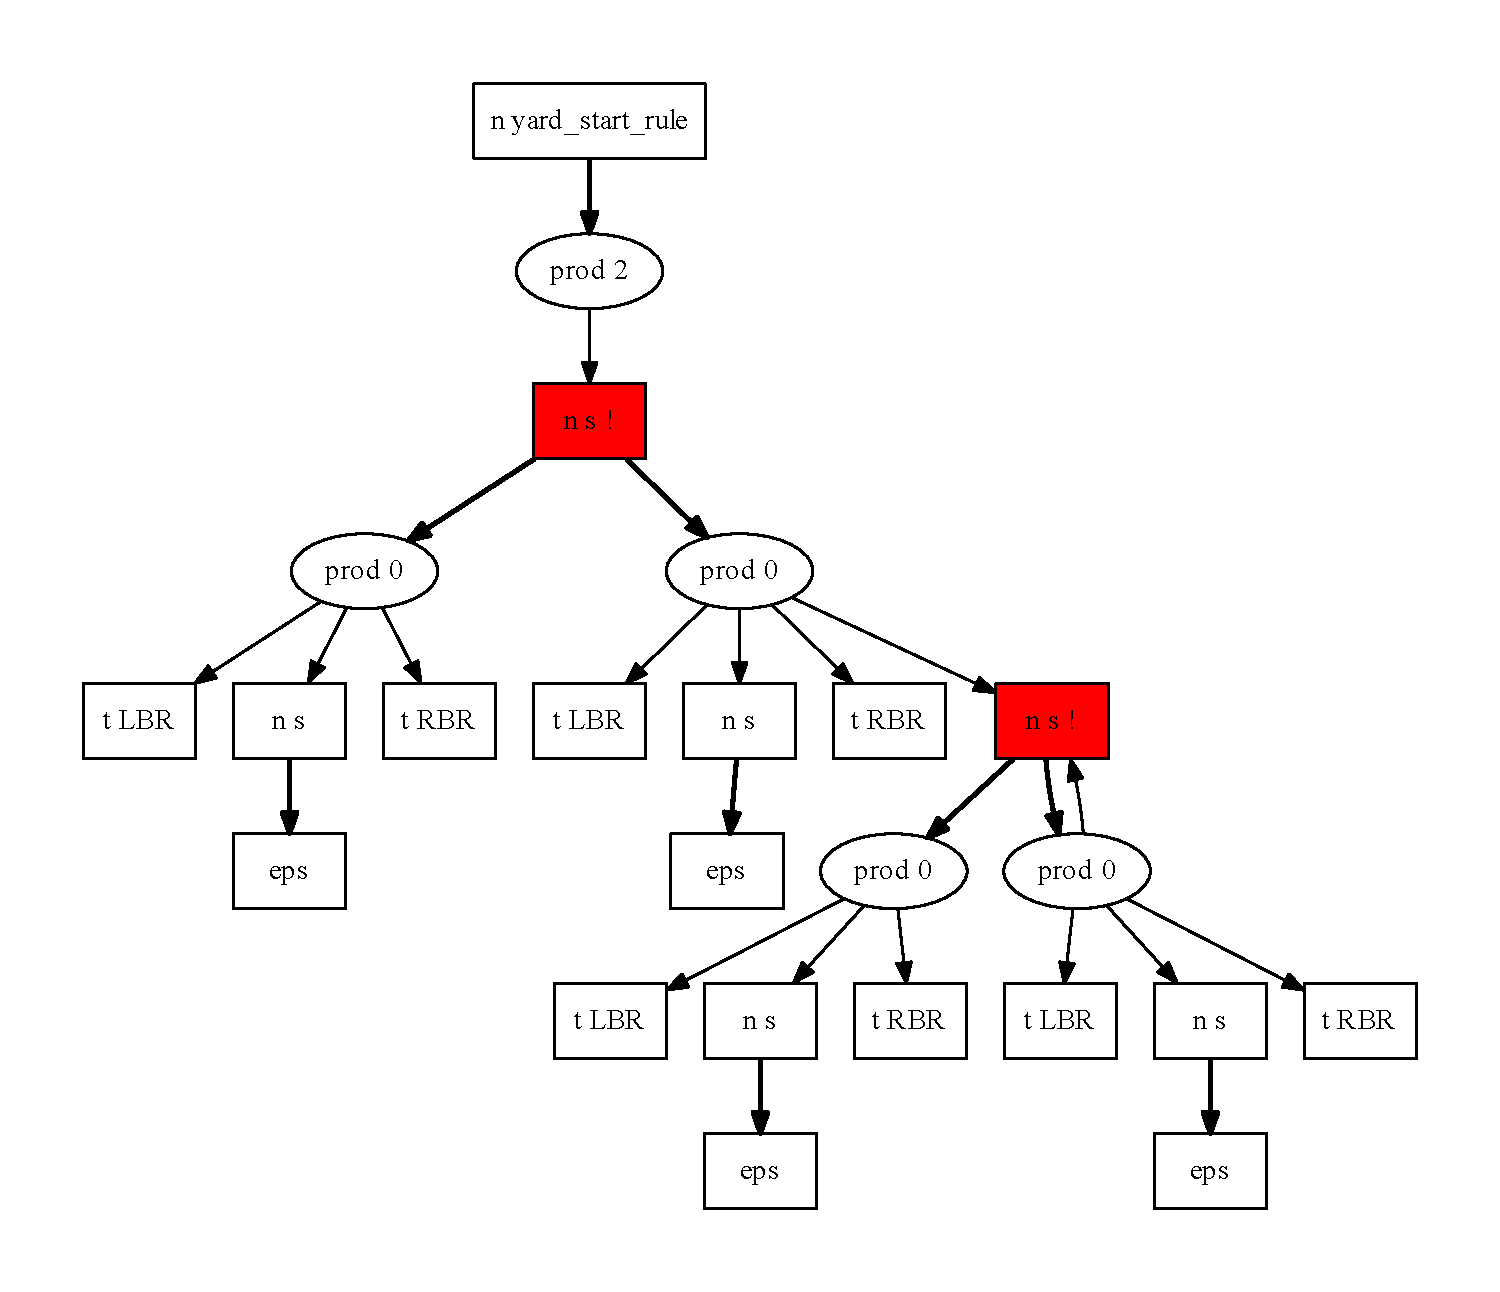
\includegraphics[width=6.8cm]{pictures/out3.pdf}}
\\
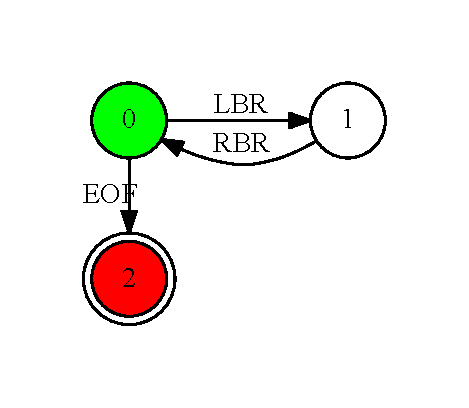
\includegraphics[width=3cm]{pictures/in3.pdf}
&
\\      
Грамматика: &
\\
\vspace{-20pt}
% Можно формулы писать
$$
\begin{array}{crcl}
&start &::=& s \\
&s & ::= & \mbox{\texttt{LBR }} s \mbox{\texttt{ RBR }} s\\
&s & ::= &\epsilon
\end{array}
$$
& 
\end{tabular}
\end{frame}

\begin{frame}[fragile]
  \frametitle{Формулировки теорем}
  \begin{rutheorem}[Пифагора: геометрическая формулировка]
    В прямоугольном треугольнике площадь квадрата, построенного на гипотенузе, равна сумме площадей квадратов, построенных на катетах.
  \end{rutheorem}

  \begin{rutheorem}[Пифагора: алгебраическая формулировка]
    В прямоугольном треугольнике квадрат длины гипотенузы равен сумме квадратов длин катетов.    

    То есть, если обозначить длину гипотенузы треугольника через $c$, а длины катетов 
через $a$ и $b$, получим верное равенство: $a^2 + b^2 = c^2$.
  \end{rutheorem}

  \begin{rutheorem}[Обратная теорема Пифагора]
    Для всякой тройки положительных чисел a, b и c, такой, что $a^2 + b^2 = c^2$, существует прямоугольный треугольник с катетами a и b и гипотенузой c.
  \end{rutheorem}  
\end{frame}

\begin{frame}[t]
  \frametitle{Экспериментальное исследование}
  \begin{itemize}
    \item На каком множестве тестов проводилось экспериментальное исследование
    \item Какие результаты показало экспериментальное исследование
    \item Желательно привести графики, иллюстрирующие полученные результаты
    \begin{itemize}
      \item У иллюстраций должны быть подписи, у графиков --- легенда, подписи к осям, например:
    \end{itemize}
  \end{itemize}
  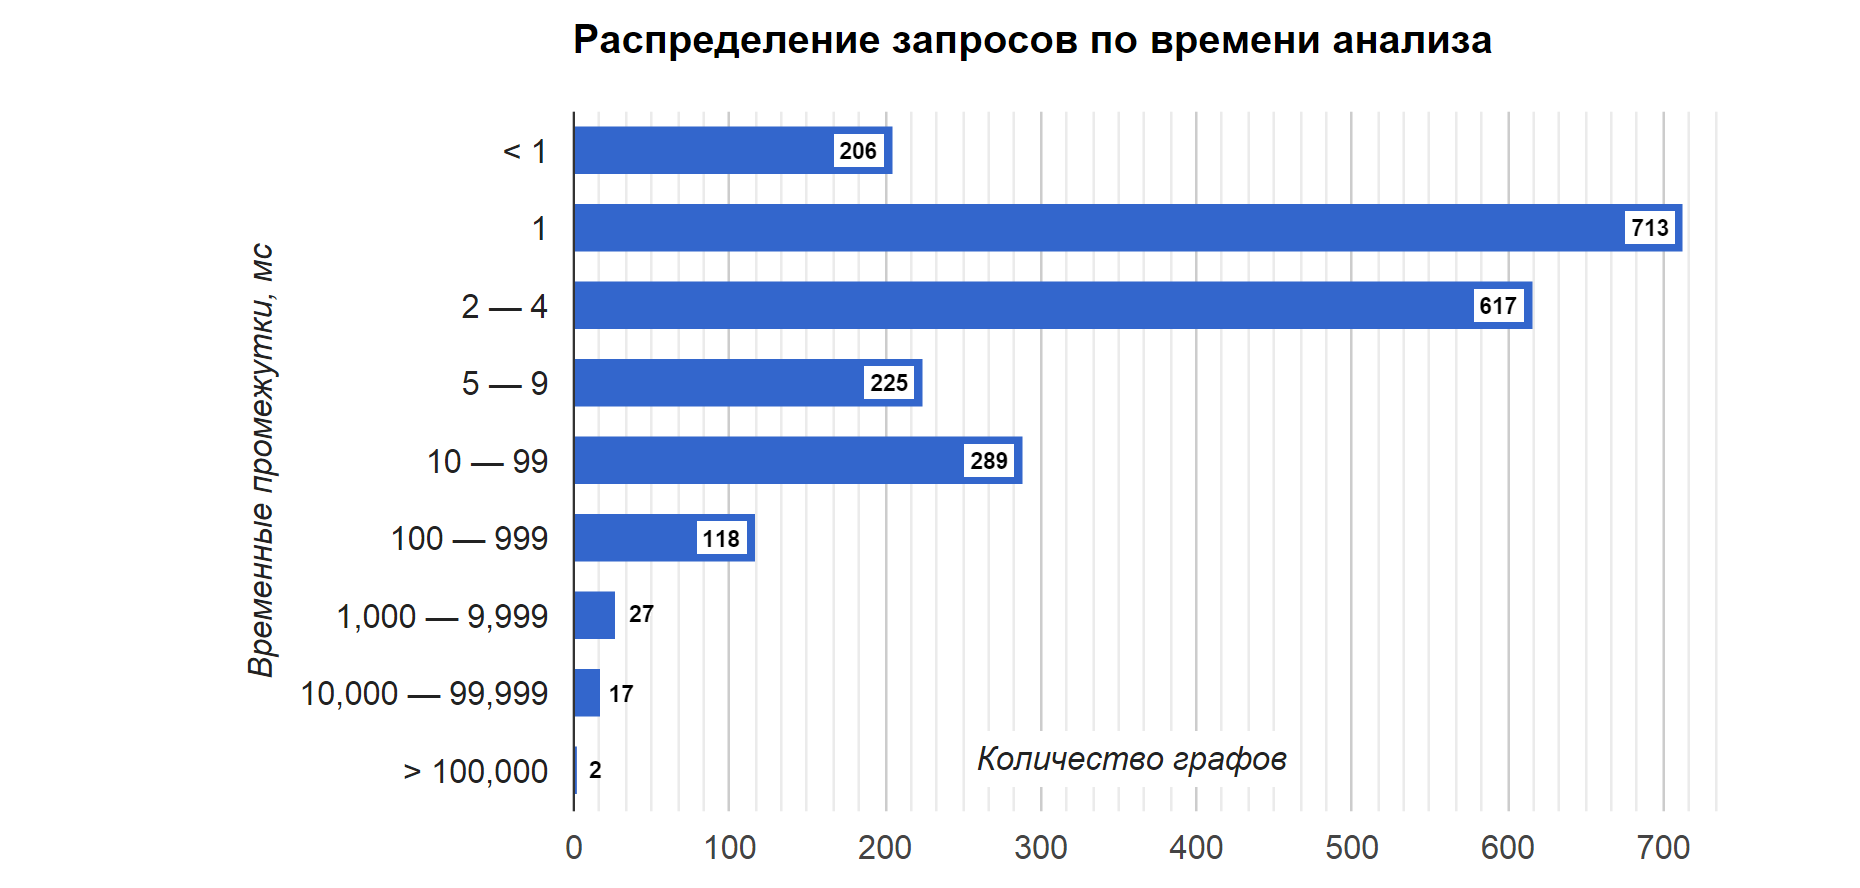
\includegraphics[width=10cm]{pictures/dist.png}
\end{frame}


\begin{frame}
  \frametitle{Результаты}
  \begin{itemize}
    \item Практически то же, что и на слайде с постановкой задачи, но в совершенной форме --- что делал лично автор
    \item Четкое отделение результатов своей работы (особенно для коллективных работ)
    \item Формулировать глаголами совершенного вида в прошедшем времени (``сделано'', ``получено'')
    \item Обсуждение (ограничения, валидность, альтернативы)
    \item Не нужно слайдов типа ``Все'', ``Вопросы?'', ``Cпасибо за внимание''
  \end{itemize}

  \begin{itemize}
    \item Если результаты были представлены на конференции и опубликованы, это желательно указать. 
  \end{itemize}
\end{frame}

%\addtocounter{framenumber}{1}
\appendix

\begin{frame}
  \frametitle{Дополнительный слайд}
  Например, с огромной страшной формулой всего, которяа нужна для пояснения деталей при ответе на частый вопрос
  
\begin{eqnarray*}
\lefteqn{
\lim_{\bigtriangleup t \to 0^+}\int_{\bigtriangleup t}^{T} \! \int_{\Omega} \! D(t_1,x) \frac{\varphi(t_1-\bigtriangleup t,x)-\varphi(t_1,x)}{(-\bigtriangleup t)} \, \mathrm{d}x \, \mathrm{d}t_1 
}\\
&=&\lim_{\bigtriangleup t \to 0^+} \int_{0}^{T} \! \int_{\Omega} \! D(t_1,x) \frac{\varphi(t_1-\bigtriangleup t,x)-\varphi(t_1,x)}{(-\bigtriangleup t)} \chi_{(\bigtriangleup t,T)}(t_1) \, \mathrm{d}x \, \mathrm{d}t_1 
\\
&= &\int_{0}^{T} \! \int_{\Omega} \! D(t_1,x) \frac{\partial \varphi}{\partial t_1} (t_1,x) \, \mathrm{d}x \, \mathrm{d}t_1 .
\end{eqnarray*}
\end{frame}

\begin{frame}
  \frametitle{Второй дополнительный слайд}

Много дополнитеьных слайдов не надо: 1--2 вполне достатчно в большинстве случаев  
  
\end{frame}

\end{document}